\documentclass[../Bachelorarbeit.tex]{subfiles}
\begin{document}

\subsection{Partitionierung}
Die Partitionierung ist der letzte Schritt der detaillierten Systemanalyse und stellt somit auch das Ende der Analysephase dar. Es schließt sich dennoch ein weiterres letztes Kapitel nachfolgend an, welches die Testspezifikationen, die im laufe der Analysephase entstanden sind, zusammenfassend dokumentiert. \\
Ziel der Partitionierung ist die Unterteilung des Systems in logische Sinnesabschnitte, um die Komplexität der Darstellung und Entwicklung zu verringern. Logische Sinnesabschnitte meint an dieser stelle jedoch nicht die logische Kontextabgrenzung aus \autoref{kontextana}, sondern ganz im Gegenteil, die physikalische Kontextabgrenzung, wie sie in \autoref{fig:my-img2} als Verteilungsdiagramm dargestellt ist. Das Verteilungsdiagramm dient als Ausgangspunkt für die Partitionierung. Nachfolgend wird die Partitionierung in drei Sinnesabschnitte unterteilt, welche in dieser Arbeit ihren eigenen Unterabschnitt erhalten. \\ % Quelle

\subsubsection{Erster Partitionierungsschritt}
In der bisherigen Betrachtung wurde das zu entwickelnde System als Black Box dargestellt. Zu erkennen sind bereits die Nachbarsysteme und die Kommunikationspfade zu diesen. \autoref{fig:my-img2} zeigt bereits Stereotypen an den Kommunikationspfaden. Dabei handelt es sich um konkrete Umsetzungen \bzw Realisierungen der Kommunikation. Aus den Realisierungen der Kommunikationspfade werden in der Partitionierung nun Schnittstellenknoten des Systems definiert. Diese sind im Folgenden in \autoref{fig:my-img10} zu erkennen. Im bisherigen Stand der Entwicklung sind nur die Stereotypen der Kommunikationspfade spezifiziert und beschreiben die Schnittstelle zu diesem. 

\begin{figure}[H]
    \centering
    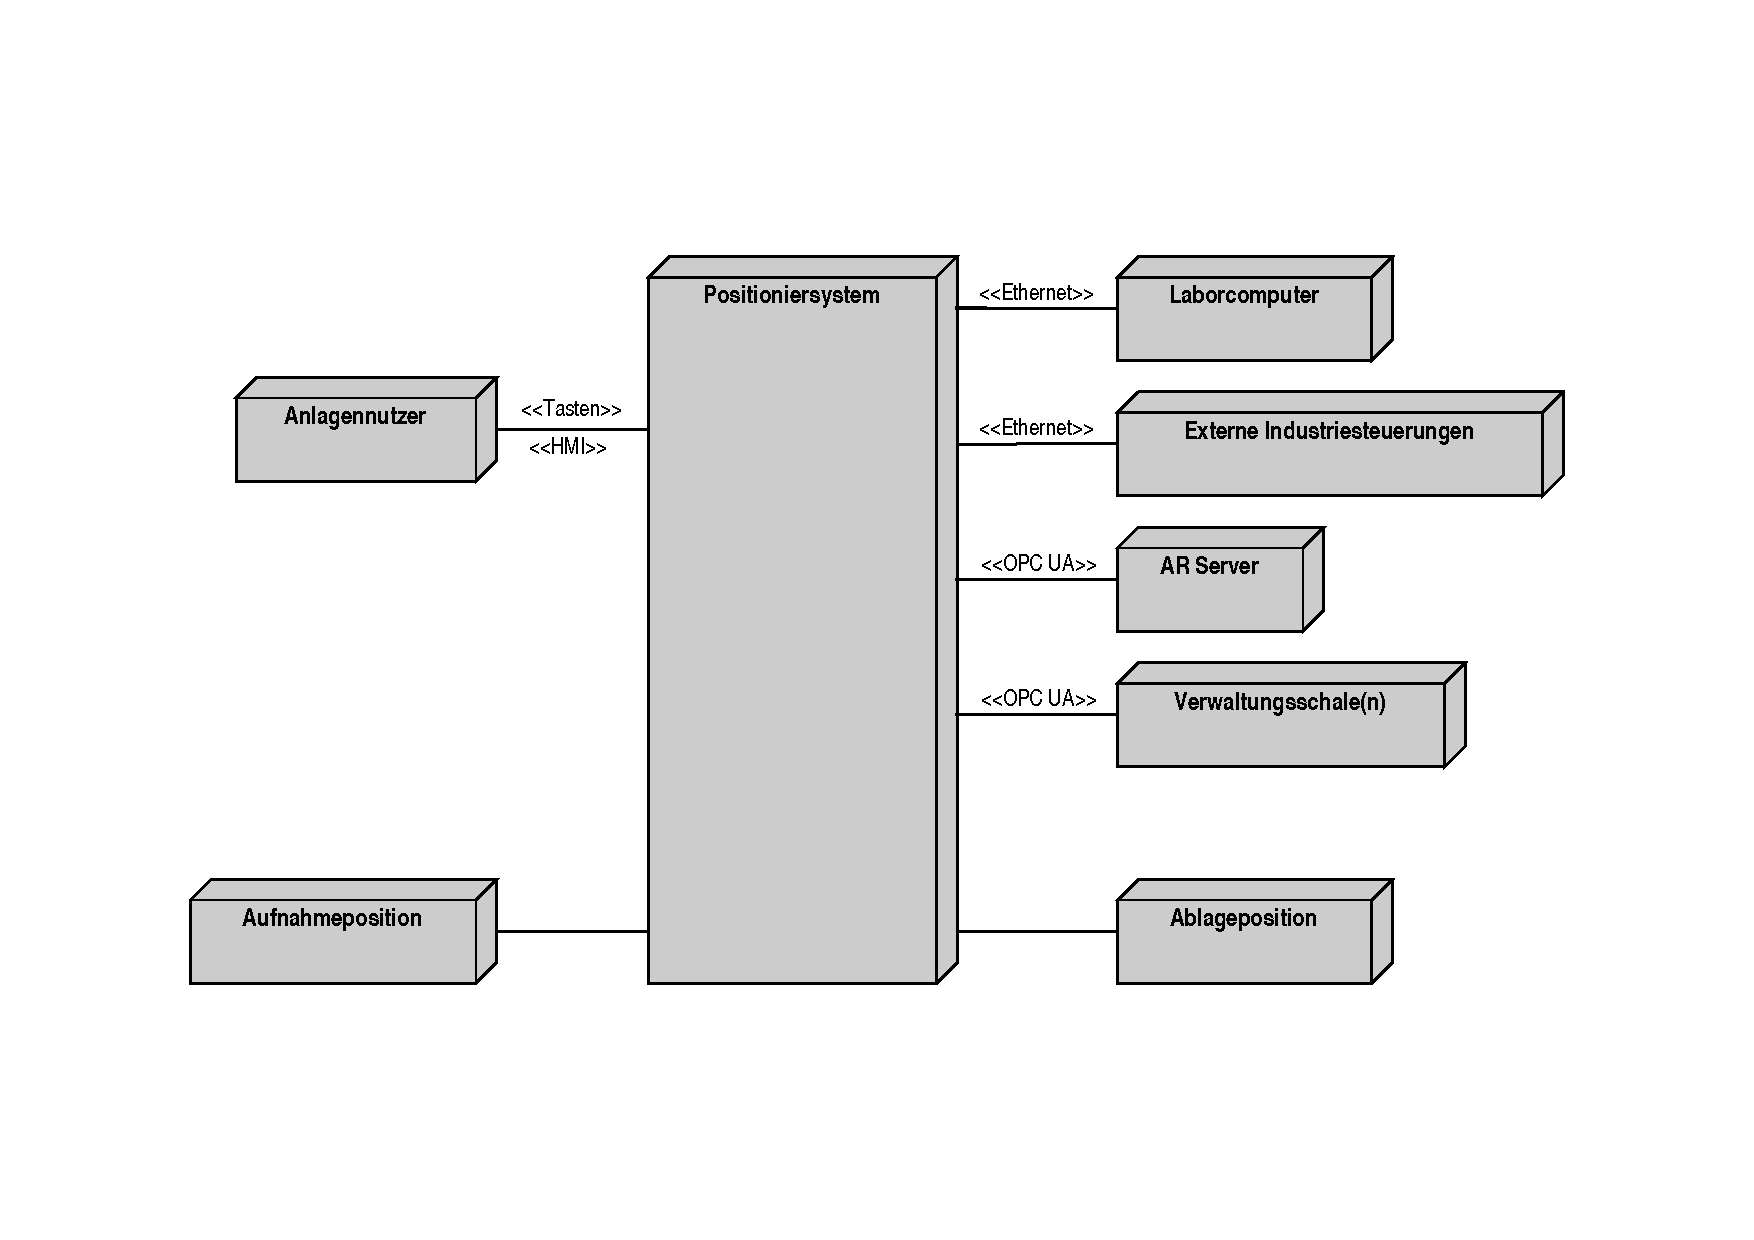
\includegraphics[width=\textwidth]{Images/phys_abgrenzung.pdf}
    \caption[Erster Partitionierungsschritt]{Erster Partitionierungsschritt}
    \label{fig:my-img10}
\end{figure}

\autoref{fig:my-img10} ergänzt zu den bereits bekannten Stereotypen, welche nun in ihren eigenen Knoten aufgeführt werden, die konkreten Knoten als Komponenten des Systems. Wichtig ist hierbei die jeweiligen Anforderungen aus \autoref{anforderungsana} zu den Knoten zu beachten.

\subsubsection{Zweiter Partitionierungsschritt}
Im zweiten Schritt wird die genaue Realisierung der Knoten und der Aufbau des Systems geklärt. Dazu werden die Systemprozessbeschreibungen aus \autoref{AnwfallSpez} benötigt. Ziel ist es das System unter funktionalen Gesichtspunkten in Komponenten \bzw Einheiten zu zerlegen. Dabei wird noch nicht festgelegt, wie die Realisierung der Einheiten mit konkreter Hardware und Software umgesetzt wird. Es findet lediglich eine Aufteilung in funktionale Komponenten statt, welche wiederum in Form von Knoten Symbolisiert werden. \\
\autoref{fig:my-img11} zeigt das entstandene Diagramm nach Anwendung der Systemprozessbeschreibungen auf die im vorherigen Unterabschnitt entwickelte Grafik. 

\begin{figure}[H]
    \centering
    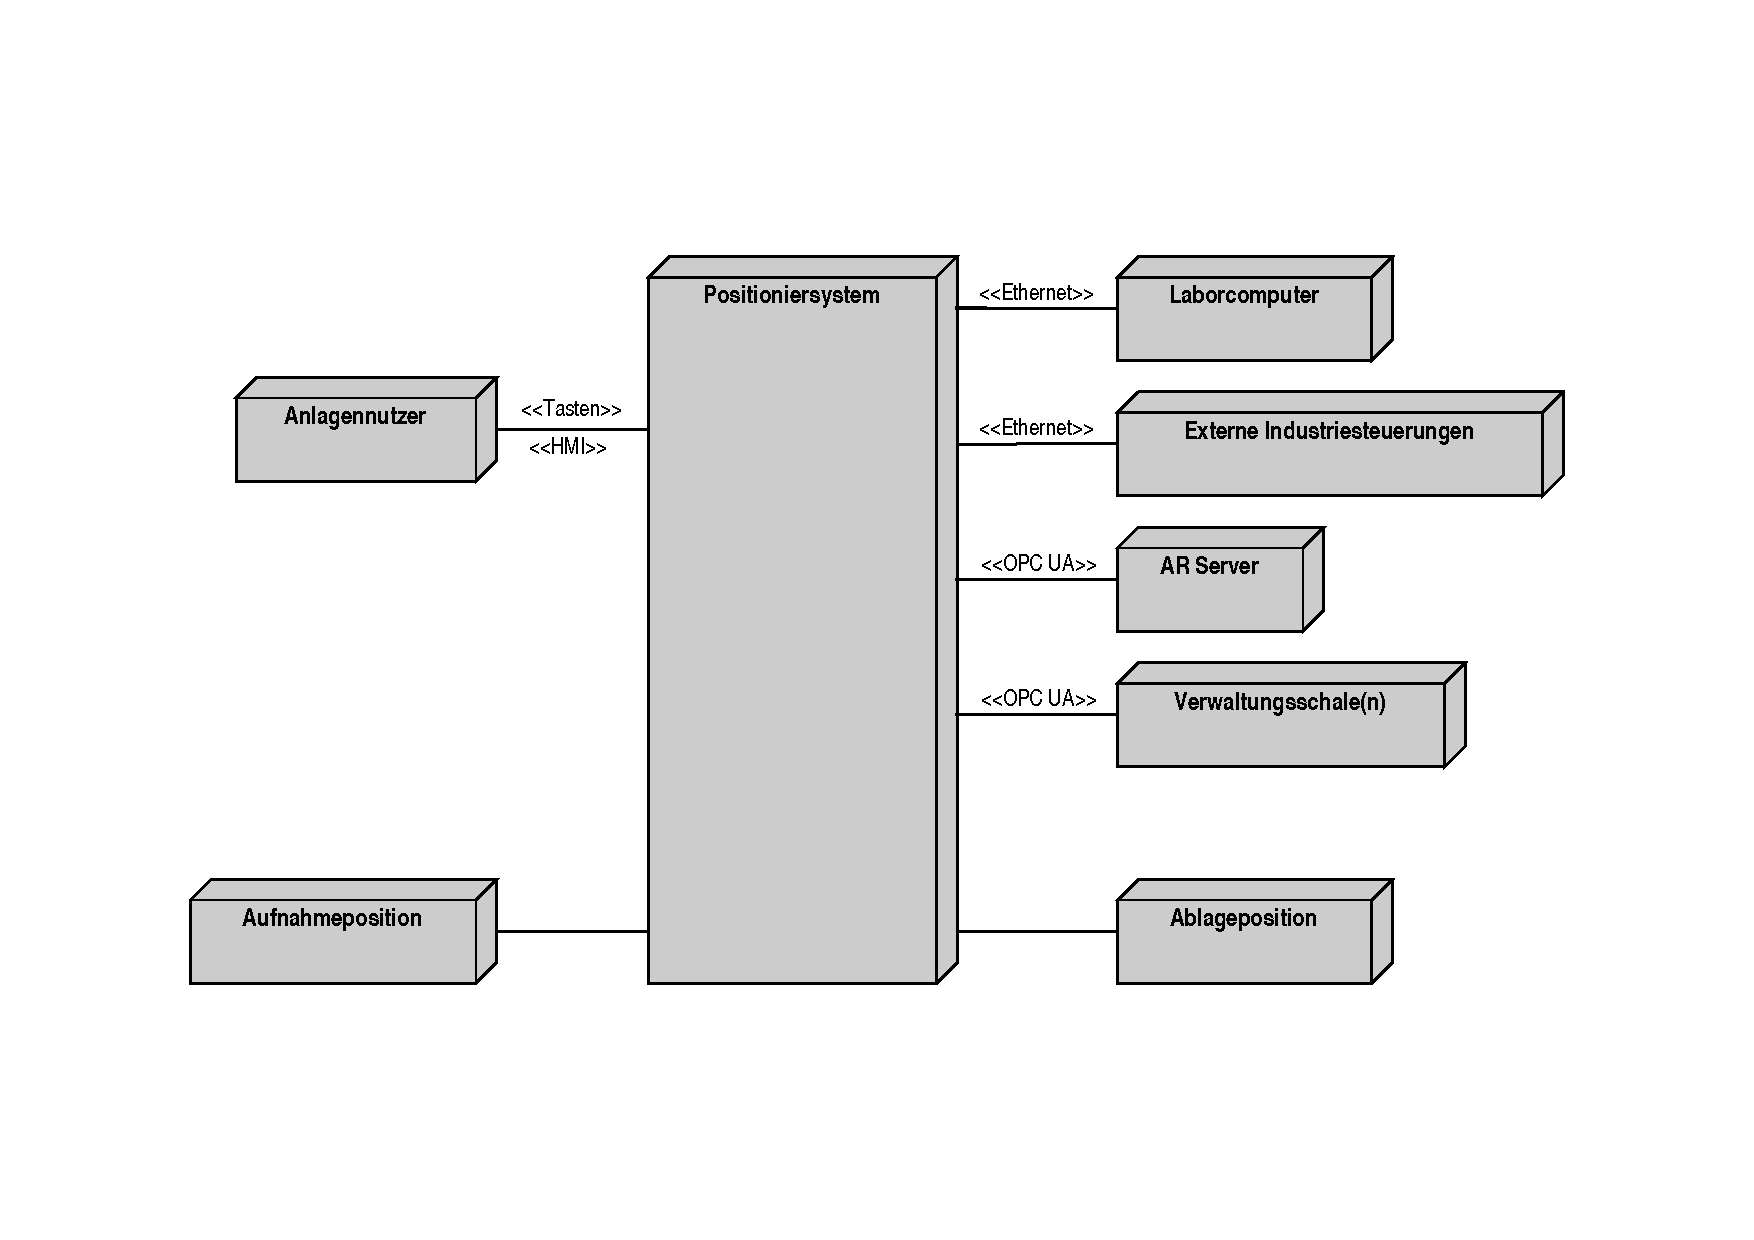
\includegraphics[width=\textwidth]{Images/phys_abgrenzung.pdf}
    \caption[Zweiter Partitionierungsschritt]{Zweiter Partitionierungsschritt}
    \label{fig:my-img11}
\end{figure}

Für diesen Partitionierungsschriit sind die \textit{essenziellen Schritte} und die \textit{Kurzbeschreibung} aus unter anderem \autoref{tab:my-table41} relevant. Für die Erstellung der kompletten Grafik müssen alle Anwendungsfallbeschreibungen berücksichtigt werden. Es fällt auf, dass im Vergleich zu Grundlegenden Anwendungsfallbeschreibung im Anwendungsfalldiagramm (\autoref{fig:my-img3}), die Betriebsmodi nicht mit aufgenommen wurden. Grund dafür ist, dass bei der Partitionierung nur die normale Arbeitsweise im Vordergrund steht. Erst bei der Realisierung der in diesem Unterabschnitt gefundenen funktionalen Knoten werden diese wieder betrachtet, da sie eigenschaften dieser Knoten beschreiben.\\
% Ergänzen mit Informationen Grafik11 und Tabelle41 ff

\subsubsection{Dritter Partitionierungsschritt}
Im dritten SChritt der Partitionierung findet eine Aufteilung der Komponenten/Einheiten in Software-, Hardware und Anlagenteil statt. Dabei ist die Aufteilung der Einheit unabhängig von der Aktuell betrachteten Einheit. Soweit es möglich ist wird die Unterteilung für jede Komponente \bzw Einheit vorgenommen. Existiert eine der drei Unterteilungen nicht für die betrachtete Einheit, entfällt diese.\\
Die \autoref{fig:my-img12} zeigt die prinzipielle Aufteilung der einzelnen Einheiten des Systems.

\begin{figure}[H]
    \centering
    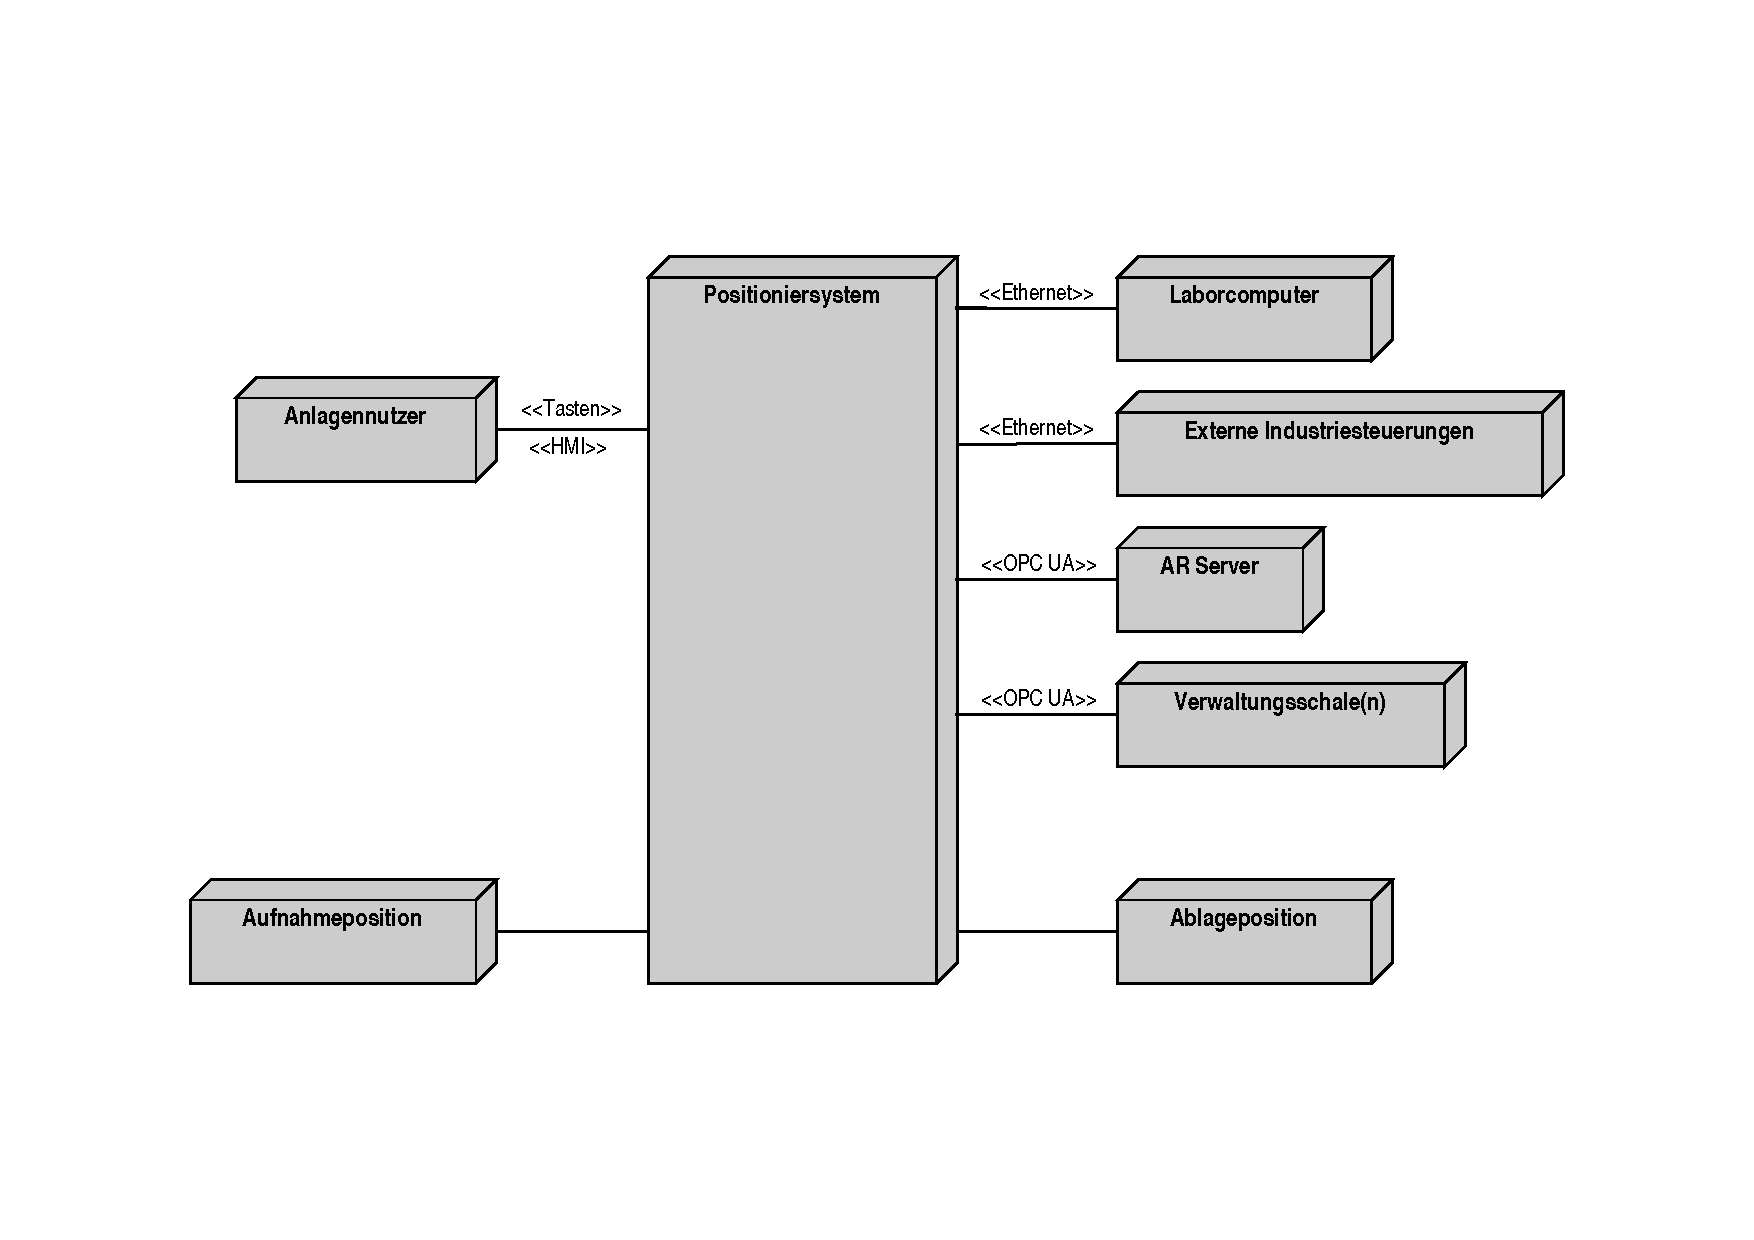
\includegraphics[width=\textwidth]{Images/phys_abgrenzung.pdf}
    \caption[Dritter Partitionierungsschritt]{Dritter Partitionierungsschritt - Aufteilungsprinzip}
    \label{fig:my-img12}
\end{figure}

Es ist zu erkennen, dass die Grafik aus drei Knoten besteht, die genau die drei Teile Anlage, Hardware und Software darstellen. Gemeinsam decken sie die Funktionalität einer Einheit ab. Ausgehend von dieser Darstellung werden nachfolgend die Schnittstellen und prinzipiellen Eigenschaften dieser Knoten entwickelt und in einer Knotenbeschreibung dokumentiert (siehe Tabelle) \\ % verlinkung hinzufügen


\end{document}